\begin{frame}
    \frametitle{Fourier Transformation}

    An absolute integrable function
    \only<-2>{$f\!: \symbb{R}\to\symbb{C}$ }
    \only<3->{$f\!: \symbb{R}^{\color{mLightBrown} N}\to\symbb{C}$ }
    can be transformed to "frequency space":
    \only<-2>{
        \begin{align*}
            \symcal{F}  [f](\nu)
            =           \hat f(\nu) = & \int_{-\infty}^{\infty} f(x) e^{-i2\pi\nu x}        \dif x   \\
            \symcal{F}^{-1}[\hat f](x)
            =           f(x)        = & \int_{-\infty}^{\infty} \hat f(\nu) e^{i2\pi\nu x}  \dif \nu
        \end{align*}
    }
    \only<3->{
        \begin{align*}
            \symcal{F}  [f](\vec\nu)
            =           \hat f(\vec\nu) =  & \int_{\color{mLightBrown}\symbb{R}^N} f(x) e^{-i2\pi{\color{mLightBrown}\vec\nu \cdot \vec x}}        \dif{}^{\color{mLightBrown}N} x  \\
            \symcal{F}^{-1}[\hat f](\vec x)
            =           f(\vec x)        = & \int_{\color{mLightBrown}\symbb{R}^N} \hat f(\nu) e^{i2\pi{\color{mLightBrown}\vec\nu\cdot \vec x}}  \dif{}^{\color{mLightBrown}N} \nu
        \end{align*}
    }

    \begin{columns}
        \begin{column}[]{.5\textwidth}

            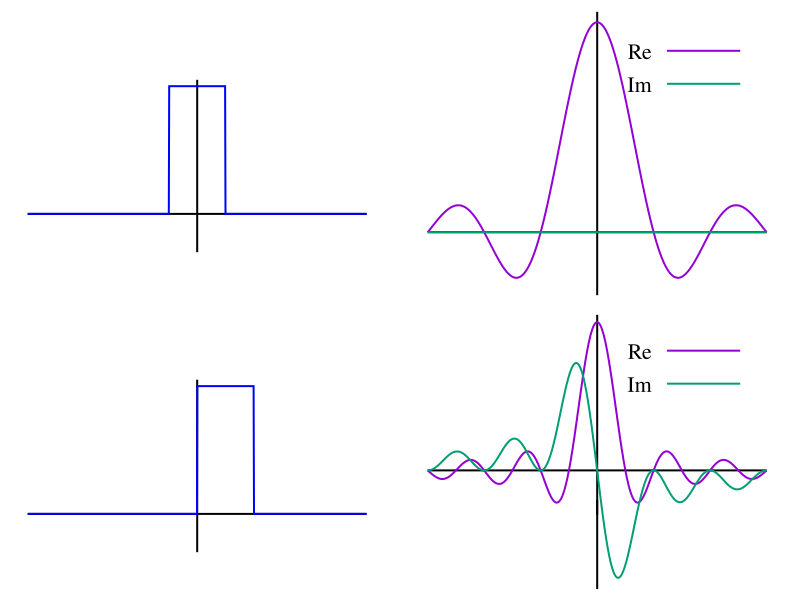
\includegraphics[trim=0 230 0 0, clip, width=\textwidth]{media/FT.png}
        \end{column}

        \begin{column}[]{.5\textwidth}

            \pause
            Important tool in physics:
            \begin{itemize}
                \item Solving differential equations
                \item Quantum mechanics: $\Psi(\vec p) = \symcal{F}[\Psi(\vec x)](\vec p)$
                \item Many more!
            \end{itemize}
        \end{column}
    \end{columns}


\end{frame}

\begin{frame}
    \frametitle{Discrete Fourier Transform}
    Let's model function, which is only nonzero at discrete values
    $0, 1, \dots, N-1$ with values proportional to $x_0, x_1, \dots, x_{N-1}$
    \begin{equation*}
        f(x) = \frac{1}{\sqrt N} \sum_{n=0}^{N-1} x_n\ \delta\left(x-{n}\right)
    \end{equation*}
    It's Fourier transform at points $0, 1/N, 2/N, \dots, N$ is the DFT of points $x_m$!
    \begin{equation*}
        \hat f\left(\frac{k}{N}\right)
        = \frac{1}{\sqrt N} \sum_{n=0}^{N-1} x_n e^{-i2\pi k \frac{n}{N}}
        = X_k
    \end{equation*}


\end{frame}

\begin{frame}
    \frametitle{(Inverse) Discrete Fourier Transform}
    \begin{equation*}
        X_k= \frac{1}{\sqrt N} \sum_{n=0}^{N-1} x_n e^{-i2\pi k \frac{n}{N}}
        \qquad \leftrightarrow \qquad
        x_k = \frac{1}{\sqrt N} \sum_{n=0}^{N-1} X_n e^{i2\pi k \frac{n}{N}}
    \end{equation*}
    \begin{columns}
        \begin{column}[]{.5\textwidth}
            \center
            \begin{tabular}{S[table-format=2.0] c<{\rightarrow} S[table-format=2.1] >{\hspace{-1em}}c<{\hspace{-.8em}} S[table-format=2.1]}
                4  &  & 44.1 & $+i$ & 0.0  \\
                8  &  & -2.4 & $+i$ & 14.8 \\
                15 &  & -9.8 & $+i$ & 9.1  \\
                16 &  & -9.8 & $+i$ & 0.0  \\
                23 &  & -9.8 & $-i$ & 9.1  \\
                42 &  & -2.4 & $-i$ & 14.8 \\
            \end{tabular}
        \end{column}
        \begin{column}[]{.5\textwidth}
            \begin{itemize}
                \item  $\symcal{F}^{-1}\left\{x_n\right\}
                          =\symcal{F}\left\{x_{N-n}\right\}
                          =\symcal{F}\left\{x_{n}^*\right\}^*$
                \item if $x_n$ real: $X_{k} = X^*_{N-k}$
            \end{itemize}
        \end{column}
    \end{columns}


\end{frame}
\begin{frame}{2D-DFT}

    \begin{equation*}
        X_{k,l} = \frac{1}{\sqrt{N_1N_2}}\sum_{n=0}^{N_1-1}\sum_{m=0}^{N_2-1}x_{n,m} \ e^{-i{2\pi}\ \left(\!\frac{kn}{N_1}+\frac{lm}{N_2}\right)}
        \qquad \leftrightarrow \qquad
        x_{k,l} = \frac{1}{\sqrt{N_1N_2}}\sum_{n=0}^{N_1-1}\sum_{m=0}^{N_2-1} X_{n,m} \ e^{i{2\pi}\ \left(\!\frac{kn}{N_1}+\frac{lm}{N_2}\right)}
    \end{equation*}

    These sums are separable:
    \begin{equation*}
        X_{k,l} =
        \frac{1}{\sqrt{N_1}}\sum_{n=0}^{N_1-1}e^{-i{2\pi}\frac{kn}{N_1}}
        \frac{1}{\sqrt{N_2}}\sum_{m=0}^{N_2-1}x_{n,m} \ e^{-i{2\pi}\frac{lm}{N_2}}
    \end{equation*}

    \color{mLightBrown}
    Perform a 2D-DFT by performing two 1D-DFT!
\end{frame}
\begin{frame}{Numerical Implementation}
    \begin{equation*}
        X_k= \frac{1}{\sqrt N} \sum_{n=0}^{N-1} x_n e^{-i2\pi k \frac{n}{N}}
    \end{equation*}
    Directly calculating this takes $N^2$ steps.
    Assuming $N$ is even, we can rewrite this as
    \begin{equation*}
        \begin{split}
            X_k &=\frac{1}{\sqrt N}
            \sum_{n=0}^{N/2-1} x_{2n} e^{-i\frac{2\pi}{N}2n k}+
            \frac{1}{\sqrt N}
            \sum_{n=0}^{N/2-1} x_{2n+1} e^{-i\frac{2\pi}{N}(2n+1) k}\\
            &= \frac{1}{\sqrt 2}
            \symcal{F}\left\{x_{2n}\right\}_k
            +\frac{1}{\sqrt 2}
            e^{-i\frac{2\pi}{N}k}\symcal{F}\left\{x_{2n+1}\right\}_k.
        \end{split}
    \end{equation*}
    We reduced the problem to about $2\cdot (N/2)^2=N^2/2$ steps.
\end{frame}
\begin{frame}{Fast Fourier Transform}
    \begin{itemize}
        \item If $N=2^p$, complexity is reduced via "Divide and Conquer" to $\symcal{O}(N\log N)$.
        \item One of the most important algorithms for modern signal processing
        \item Rediscovered and popularized by Cooley and Tukey in 1965\footnote{\fullcite{CTAlg}}
        \item Described in notes of Gauss 160 years(!) earlier
    \end{itemize}
\end{frame}
\begin{frame}{FFT of arbitrary size?}
    The Algorithm by Cooley-Tukey  works for every composite size $N=N_1\cdot N_2$

    What if $N$ is prime?
    \pause

    Then the set of numbers $G=\{0, 1, 2, \dots, N-1\}$ form a group with $\circ: G\times G\to G$
    \begin{equation*}
        a\circ b = a\cdot b\quad \symup{mod}\ N
    \end{equation*}
    DFT can then be expressed as a convolution. \emph{Rader's} Algorithm uses this to achieve $\symcal{O}(N\log N)$
\end{frame}